%%%%%%%%%%%%%%%%%%%%%%%%%%%%%%%%%%%%%%%%%%%%%%%%%
\section[Reconstruction]{Reconstruction}
%------------------------------------------------
%++++++++++++++++++++++++++++++++++++++++++++++++
\subsection{Détermination du système}
%++++++++++++++++++++++++++++++++++++++++++++++++

\begin{frame}
\frametitle{Les différents repères}

\begin{minipage}{0.48\textwidth}
    \centering
    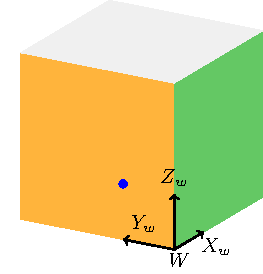
\includegraphics[width=\linewidth]{capture/cube_tikz.pdf}
    \vspace{0.5em}
    
    {\footnotesize\textbf{Représentation du cube (vue 3D)}}
\end{minipage}
\hfill
\begin{minipage}{0.48\textwidth}
    \centering
    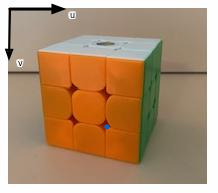
\includegraphics[width=\linewidth]{capture/cube_repere.png}
    \vspace{0.5em}

    {\footnotesize\textbf{Cube sur une image}}
\end{minipage}

\end{frame}

\begin{frame}{Modèle de projection — Matrice \( P \)}

\begin{itemize}
  \note{sans entrer dans les détails du calcul, on montre qu on peut lié les coordonnées réels et sur l image par une relation homogene (homgene car la projection nous fait perdre une dimension)
  matrice de projection encode les caractéristiques de la caméra (rotation et translation) et les parametresintrinsèque (distance focale, taille des pixels)}
  \item<1-> On considère un point 3D \( M = (X, Y, Z) \)
  \item<2-> Il se projette sur un point image \( m = (u, v) \)
  \hyperlink{projection-appendix}{
    \beamerbutton{Compléments projections}
  }
  \item<3-> On cherche une relation linéaire homogène :
  \[
  \lambda
  \begin{bmatrix}
  u \cr v \cr 1
  \end{bmatrix}
  P
  =
  \begin{bmatrix}
  X \cr Y \cr Z \cr 1
  \end{bmatrix}
  \]

  \item<4-> \( P \) est une matrice \( 3 \times 4 \), avec 12 inconnues
  \item<5-> En faisant cela pour 6 points on obtient un système ...
\end{itemize}
\end{frame}

%------------------------


\begin{frame}{Système matriciel}
  
\[
\resizebox{\textwidth}{!}{$
\left(
\begin{array}{cccccccccccc}
    x_{C}^{(1)} & y_{C}^{(1)} & z_{C}^{(1)} & 1 & 0 & 0 & 0 & 0 & -u^{( 1)} x{C}^{(1)} & -u^{( 1)}y{C}^{(1)} & -u^{( 1)}z_{C}^{(1)} & -u^{(1)}\\
0 & 0 & 0 & 0 & x_{C}^{( 1)} & y_{C}^{( 1)} & z_{C}^{( 1)} & 1 & -v^{( 1)} x_{C}^{( 1)} & -v^{( 1)} y_{C}^{( 1)} & -v^{( 1)} z_{C}^{( 1)} & -v^{( 1)}\\
\vdots  & \vdots  & \vdots  & \vdots  & \vdots  & \vdots  & \vdots  & \vdots  & \vdots  & \vdots  & \vdots  & \vdots \\
x_{C}^{( i)} & y_{C}^{( i)} & z_{C}^{( i)} & 1 & 0 & 0 & 0 & 0 & -u^{( i)} x_{C}^{( i)} & -u^{( i)} y_{C}^{( i)} & -u^{( i)} z_{C}^{( i)} & -u^{( i)}\\
0 & 0 & 0 & 0 & x_{C}^{( i)} & y_{C}^{( i)} & z_{C}^{( i)} & 1 & -v^{( i)} x_{C}^{( i)} & -v^{( i)} y_{C}^{( i)} & -v^{( i)} z_{C}^{( i)} & -v^{( i)}\\
\vdots  & \vdots  & \vdots  & \vdots  & \vdots  & \vdots  & \vdots  & \vdots  & \vdots  & \vdots  & \vdots  & \vdots \\
x_{C}^{( 6)} & y_{C}^{( 6)} & z_{C}^{( 6)} & 1 & 0 & 0 & 0 & 0 & -u^{( 6)} x_{C}^{( 6)} & -u^{( 6)} y_{C}^{( 6)} & -u^{( 6)} z_{C}^{( 6)} & -u^{( 6)}\\
0 & 0 & 0 & 0 & x_{C}^{( 6)} & y_{C}^{( 6)} & z_{C}^{( 6)} & 1 & -v^{( 6)} x_{C}^{( 6)} & -v^{( 6)} y_{C}^{( 6)} & -v^{( 6)} z_{C}^{( 6)} & -v^{( 6)}
\end{array}
\right)
\begin{pmatrix}
p_{11}\\
p_{12}\\
p_{13}\\
p_{14}\\
p_{21}\\
p_{22}\\
p_{23}\\
p_{24}\\
p_{31}\\
p_{32}\\
p_{33}\\
p_{34}
\end{pmatrix} =\begin{pmatrix}
0\\
0\\
0\\
0\\
0\\
0\\
0\\
0\\
0\\
0\\
0\\
0
\end{pmatrix}
$}
\]
\end{frame}


\begin{frame}{Calibration}
  \note{
    1. Rubik's Cube comme mire de calibrage,\\
    permet d'identifier facilement les faces et d'y apposer un repère.\\
    On crée des fichiers types avec les coordonnées des points pour chaque paire de faces,\\
    et il suffit de sélectionner les points à la main pour calibrer.
  }
  \centering
  \begin{minipage}{0.32\linewidth}
    \centering
    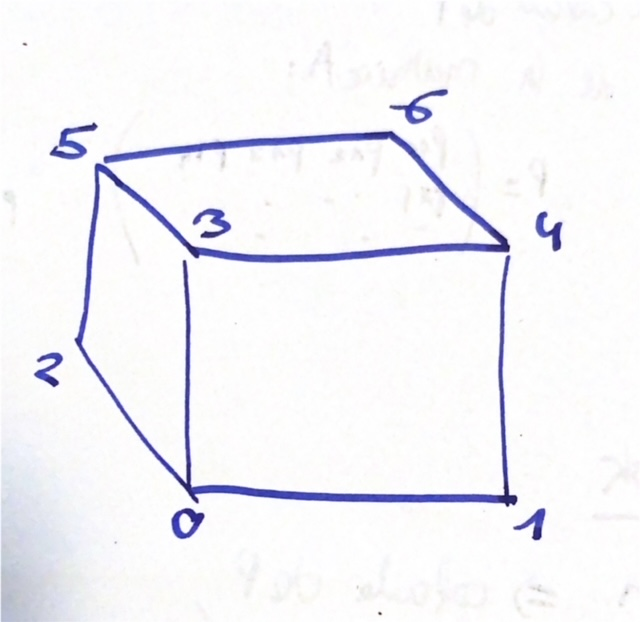
\includegraphics[width=0.9\linewidth]{capture/cube_tuto.JPG}
    \vspace{1cm}
    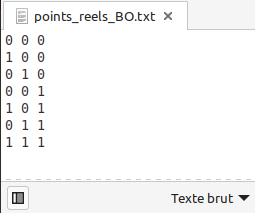
\includegraphics[width=0.9\linewidth]{capture/BO.png}
  \end{minipage}
  \hfill
  \begin{minipage}{0.6\linewidth}
    \centering
    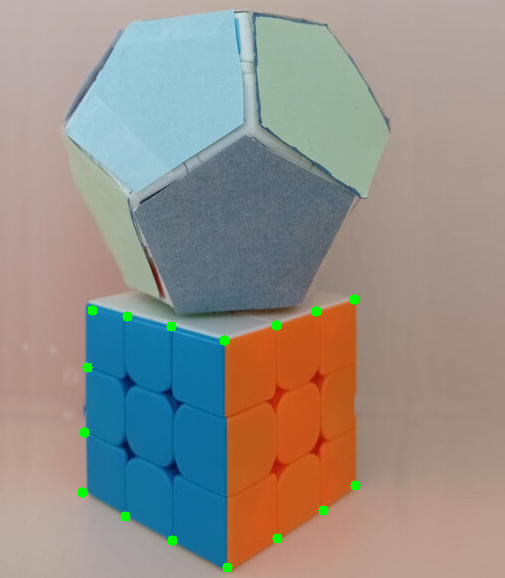
\includegraphics[width=0.9\linewidth]{capture/selection.png}
    \captionof{figure}{Interface utilisateur}
  \end{minipage}
\end{frame}
